\chapter{\label{chap:lit-review}Revisão Bibliográfica}

\section{SpelunkBots} TBD

\subsection{Spelunky}
% Colocar uma foto ilustrativa em algum lugar Falar mais sobre as áreas?  Falar
% mais sobre os itens?
Spelunky \cite{SPELUNKYWEB} é um jogo onde o jogador incorpora um aventureiro
que decide explorar uma caverna misteriosa. O local contém tesouros fabulosos,
mas também está repleto de perigos. O objetivo principal do jogador é explorar
estes túneis subterrâneos e coletar a maior quantia de tesouros possível
enquanto evita ser abatido pelos diversos inimigos e armadilhas espalhadas pelo
ambiente. O jogo 2D\footnote{Jogo Bidimensional, ou seja, trabalha-se em apenas
duas dimensões. Muitas vezes, contudo, perspectiva e profundidade são geradas de
maneira ilusória.} segue o estilo \textit{platformer}\footnote{Estilo de jogo
que envolve guiar um personagem através de plataformas suspensas e obstáculos
para obter progresso no jogo.} e emprega alguns elementos do gênero
\textit{roguelike}, como geração procedural\footnote{Técnica utilizada para
gerar dados algoritmicamente ao invés de manualmente. Em jogos digitais, pode
ser utilizado para criar conteúdo de forma automática.} e morte permanente.

O jogo é dividido em 4 áreas principais: \textbf{As Minas}, \textbf{A Selva},
\textbf{As Cavernas De Gelo} e \textbf{O Templo}. Cada área possúi um estilo de
mapa e aparência única. O nível de dificuldade também aumenta gradativamente,
principalmente porque os inimigos vão se tornando cada vez mais fortes. Além das
áreas principais, existem duas áreas secretas: \textbf{O Mercado Negro} e
\textbf{A Cidade de Ouro}.

O jogador, inicialmente, conta somente com um chicote, 4 pontos de vida, 4
bombas e 4 cordas para ajudá-lo a se defender e se locomover pela caverna.
Contudo, diversos equipamentos, acessórios e armas podem ser obtidos e
utilizados ao longo do jogo. Além disso, o jogador pode interagir com objetos do
ambiente, como pedras, vasos, baús de tesouro, entre outros. Também se
encontram, espalhados pelas cavernas, os \textbf{Comerciantes}. Estes
\textit{NPCs}\footnote{\textit{Non-Playable Characters}(Personagens
Não-Jogáveis). São personagens que não são controlados pelo jogador. Geralmente
interagem de alguma maneira com o personagem do jogador.} comercializam itens
com o jogador em troca de tesouros. É possível, inclusive, tentar furtar itens
destes comerciantes. Contudo, se o jogador o fizer, todos os comerciantes
ficarão extremamente irritados e passarão a caçar o explorador com espingardas.

Os níveis em Spelunky são gerados proceduralmente, fazendo com que cada partida
seja única. Isto significa que não existe uma maneira de se ``decorar'' Spelunky,
pois ao início de cada partida o mapa é gerado de maneira única e os tesouros,
itens e obstáculos são dispostos de maneira diferente, fazendo com que o jogador
tenha que aprender a lidar com os elementos de forma individual, combinar este
conhecimento e estabelecer uma estratégia para vencer seus obstáculos e ser bem
sucedido.

O jogo foi desenvolvido por Derek Yu - utilizando o motor de desenvolvimento de
jogos \textit{GameMaker} (Versão 8) - e lançado gratuitamente para a plataforma
\textit{Windows} em dezembro de 2008\cite{SPELUNKYRELEASE}. No fim de 2009, o
criador optou por liberar o código fonte do jogo, permitindo sua distribuição
não-comercial e modificação\cite{SPELUNKYLICENSE}.

O uso do GameMaker para o desenvolvimento do jogo faz com que seja possível o
uso de ferramentas que facilitam o trabalho do desenvolvedor. Contando com
funcionalidades como editores de \textit{scripts}\footnote{Código desenvolvido
para o controle dos comportamentos dos elementos do jogo.} e de
\textit{sprites}\footnote{Elementos visuais do jogo, tais como o personagem, o
fundo, os inimigos. Representados como uma ou mais imagens, permitindo que as
mesmas sejam animadas.}, gerenciadores de eventos, entre outras
\cite{GMAKER8DOCS}, o GameMaker oferece um ótimo suporte ao desenvolvedor para
a criação de jogos.

\begin{figure}[htb!]
\centering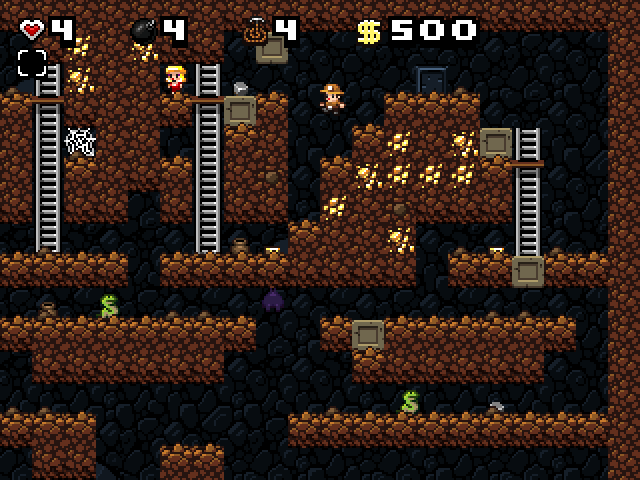
\includegraphics[width=.65\textwidth]{fig/spelunky-pc-screen.png}
\caption
    {\label{fig:spelunky-gameplay}Exemplo de partida de spelunky, mostrando
    elementos do jogo como o jogador, a caverna, os inimigos, os tesouros,
    entre outros.}
\end{figure}

\subsection{Competição SpelunkBots}
% O framework A competição

TBD

\section{Agentes Racionais}

Um agente pode ser visto como todo e qualquer tipo de entidade que seja capaz de
perceber o ambiente onde está situado, através de seus sensores, podendo
executar ações nesse ambiente conforme sua necessidade através de seus
atuadores.
\cite{Russell:1995:AIM:193191}

Para exemplificar, podemos tomar como exemplo o ser humano, que consegue
perceber o ambiente através de seus olhos e ouvidos, por exemplo, conseguindo
agir no ambiente com suas partes do corpo, como braços, pernas, mãos e etc.
\cite{Russell:1995:AIM:193191}

Nesse contexto, um agente racional é um agente que toma as ações que o coloca
mais próximo de completar seus objetivos.

\subsection{Agentes Reflexivos}

TBD

\subsection{Agentes com Memória}

TBD

\subsection{Agentes Baseados em Objetivos}

TBD

\subsection{Agentes Baseados em Utilidades}

TBD

\subsection{Ambiente}

TBD

\subsection{Objetivo}

TBD

\subsection{Estado}

TBD

\subsection{Agentes BDI}

TBD

\section{Frameworks de Inteligência Artificial}

TBD

\subsection{Motivação}

TBD

\subsection{Exemplos de Frameworks e Competições}

TBD

\section{Planejamento}

TBD

\section{Aprendizado de Máquina}

TBD

\subsection{Q-Learning}

TBD

\subsection{SARSA}

TBD

\subsection{Deep Learning}

TBD
